\documentclass{article}
\usepackage[utf8]{inputenc}
\usepackage{amsmath}
\usepackage{amsfonts}
\usepackage{amssymb}
\usepackage{geometry}
\usepackage{listings}
\usepackage{xcolor}
\usepackage{caption}
\usepackage{enumitem}
\usepackage{graphicx}
\geometry{a4paper, margin=1in}

\definecolor{codegreen}{rgb}{0,0.6,0}
\definecolor{codegray}{rgb}{0.5,0.5,0.5}
\definecolor{codepurple}{rgb}{0.58,0,0.82}
\definecolor{backcolor}{rgb}{0.95,0.95,0.92}

\lstdefinestyle{mystyle}{
    backgroundcolor=\color{backcolor},
    commentstyle=\color{codegreen},
    keywordstyle=\color{magenta},
    numberstyle=\tiny\color{codegray},
    stringstyle=\color{codepurple},
    basicstyle=\footnotesize,
    breakatwhitespace=false,
    breaklines=true,
    captionpos=b,
    keepspaces=true,
    numbers=left,
    numbersep=5pt,
    showspaces=false,
    showstringspaces=false,
    showtabs=false,
    tabsize=2
}

\lstset{style=mystyle}

\title{Basic Probability and Its Applications in AI}
\author{Tai Bui Van, Cuong Tran Xuan, An Bui Hoang, Khanh Nguyen Nam, Anh Nguyen Thi Lan}
\date{}
\begin{document}

\maketitle
Probability helps us understand uncertainty and make predictions.
In this document, we'll learn basic probability concepts and see how they are used in artificial intelligence.

\section*{1. Introduction}

\subsection*{Experiment and Event}

An \textbf{experiment} is any procedure that can be repeated multiple times under the same conditions and has a well-defined set of possible outcomes.
The set of all possible outcomes is called the \textbf{sample space}, usually denoted by $\Omega$ or $S$.

An \textbf{event} is a subset of the sample space - it's a collection of possible outcomes that we're interested in. Events are typically denoted by capital letters like $A$, $B$, etc.

\textbf{Example:}
Consider the experiment of rolling a six-sided dice. In this case:

\begin{itemize}
    \item The \textbf{experiment} is the act of rolling the dice
    \item The \textbf{sample space} $\Omega = \{1, 2, 3, 4, 5, 6\}$ contains all possible outcomes
    \item Some examples of \textbf{events} could be:
    \begin{itemize}
        \item Event $A$: Rolling an odd number = $\{1, 3, 5\}$
        \item Event $B$: Rolling a even number = $\{2, 4, 6\}$
        \item Event $C$: Rolling a prime number = $\{2, 3, 5\}$
    \end{itemize}
\end{itemize}

Each time we perform this experiment, exactly one outcome from the sample space will occur. An event is said to occur if the actual outcome is one of the outcomes in that event's set.

\begin{figure}[h]
    \centering
    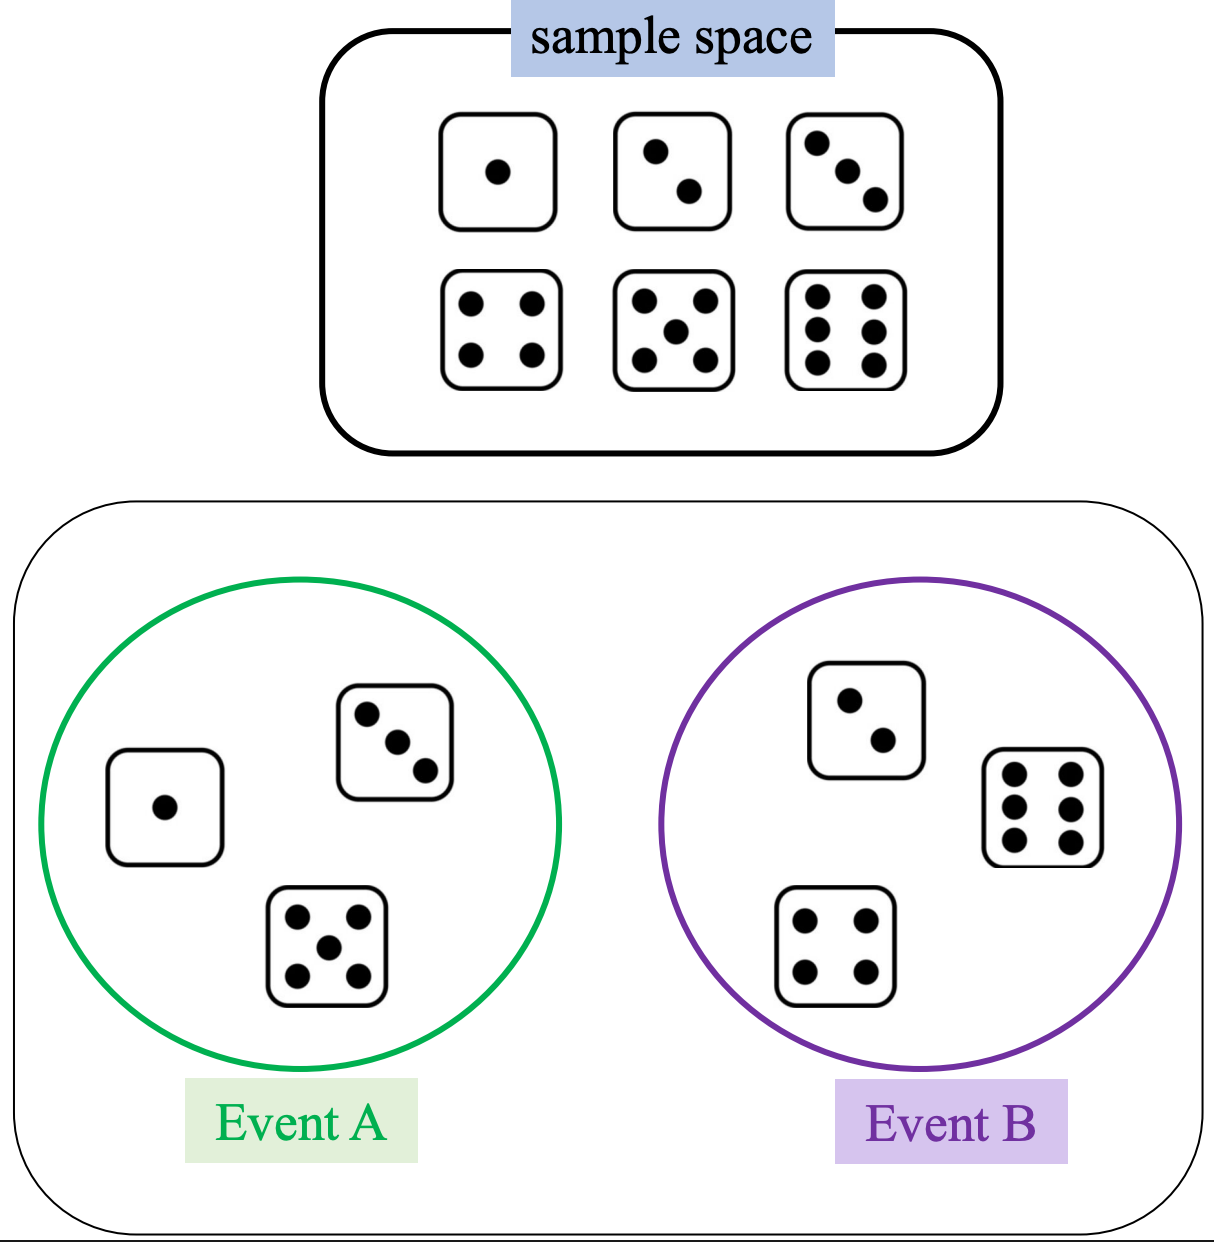
\includegraphics[width=0.5\textwidth]{images/image1.png}
    \caption{Example of Experiment and Event}
    \label{fig:experiment-event}
\end{figure}

\subsection*{Operations on Event \& Relations of Event}

\subsubsection*{Union of Events:}
The union of two events $A$ and $B$, denoted $A \cup B$, is the event that occurs if either $A$ or $B$ or both occur.

\textbf{Example:}

\begin{align*}
    A &= \{1, 3, 5\} \\
    B &= \{2, 4, 6\} \\
    A \cup B &= \{1, 2, 3, 4, 5, 6\}
\end{align*}


\subsubsection*{Intersection of Events:}
The intersection of two events $A$ and $B$, denoted $A \cap B$, is the event that occurs if both $A$ and $B$ occur.

\textbf{Example:}
\begin{align*}
    A &= \{1, 3, 5\} \\
    B &= \{2, 4, 6\} \\
    A \cap B &= \{2, 4, 6\}
\end{align*}

\subsubsection*{Complementary Event:}
The complementary event of an event $A$, denoted $A^c$, is the event that occurs if $A$ does not occur.

\textbf{Example:}
\begin{align*}
    A &= \{1, 3, 5\} \\
    A^c &= \{2, 4, 6\}
\end{align*}


\subsubsection*{Mutually Exclusive Events:}
Two events $A$ and $B$ are mutually exclusive if they cannot occur at the same time, i.e., $A \cap B = \emptyset$.

\textbf{Example:}
\begin{align*}
    A &= \{1, 3, 5\} \\
    B &= \{2, 4, 6\} \\
    A \cap B &= \emptyset
\end{align*}

\subsection*{Disjoint Events}
Two events $A$ and $B$ are disjoint if they cannot occur at the same time, i.e., $A \cap B = \emptyset$.

\textbf{Example:}
\begin{align*}
    A &= \{\text{getting heads}\} \\
    B &= \{\text{getting tails}\} \\
    A \cap B &= \emptyset
\end{align*}


\section*{2. Probability \& Bayes' Rule}

\subsection*{Classical Definition of Probability}

The probability of an event $A$ is defined as the ratio of the number of favorable outcomes to the total number of possible outcomes.

\begin{align*}
    P(A) &= \frac{\text{number of favorable outcomes}}{\text{total number of possible outcomes}}
\end{align*}


For example, when rolling a fair six-sided die:

\begin{itemize}
    \item The probability of getting an even number is:
    $$P(\text{even}) = \frac{|\{2,4,6\}|}{|\{1,2,3,4,5,6\}|} = \frac{3}{6} = \frac{1}{2}$$

    \item The probability of getting a number greater than 4 is:
    $$P(>4) = \frac{|\{5,6\}|}{|\{1,2,3,4,5,6\}|} = \frac{2}{6} = \frac{1}{3}$$
\end{itemize}

This definition assumes that all outcomes are equally likely (uniform probability distribution). In many real-world scenarios, this assumption may not hold true, leading us to consider empirical or subjective probabilities.

\subsection*{Empirical probability (experimental probability)}

\subsection*{Rules of Probability}

\subsubsection*{Addition Rule:}
The probability of the union of two events $A$ and $B$ is given by:

$$
P(A \cup B) = P(A) + P(B) - P(A \cap B)
$$

\subsubsection*{Multiplication Rule:}
The probability of the intersection of two events $A$ and $B$ is given by:

$$
P(A \cap B) = P(A) \cdot P(B \mid A)
$$

\subsubsection*{Conditional Probability:}
The probability of an event $A$ given that event $B$ has occurred is given by:

$$
P(A \mid B) = \frac{P(A \cap B)}{P(B)}
$$


\subsection*{Total Probability}

The law of total probability states that for any event $A$ and a partition of the sample space $\{B_1, B_2, ..., B_n\}$:

$$
P(A) = \sum_{i=1}^n P(A|B_i)P(B_i)
$$

This is particularly useful when it's easier to compute conditional probabilities $P(A|B_i)$ than to compute $P(A)$ directly.

\subsubsection*{Example}
Consider a company that produces electronic components. The components are manufactured in three different factories:
\begin{itemize}
    \item Factory 1 produces 50\% of the components with a 3\% defect rate
    \item Factory 2 produces 30\% of the components with a 2\% defect rate
    \item Factory 3 produces 20\% of the components with a 4\% defect rate
\end{itemize}

The probability of getting a defective component can be calculated using the law of total probability:

\begin{align*}
P(\text{defective}) &= P(\text{defective}|F_1)P(F_1) + P(\text{defective}|F_2)P(F_2) + P(\text{defective}|F_3)P(F_3) \\
&= (0.03)(0.5) + (0.02)(0.3) + (0.04)(0.2) \\
&= 0.015 + 0.006 + 0.008 \\
&= 0.029 \text{ or } 2.9\%
\end{align*}

\subsection*{Bayes' Rule}
Bayes' rule is a fundamental theorem in probability theory that allows us to update our beliefs based on new evidence.

Bayes' rule states that:

$$
P(A|B) = \frac{P(B|A)P(A)}{P(B)}
$$

where:
\begin{itemize}
    \item $P(A|B)$ is the posterior probability of $A$ given $B$
    \item $P(B|A)$ is the likelihood of $B$ given $A$
    \item $P(A)$ is the prior probability of $A$
    \item $P(B)$ is the probability of $B$
\end{itemize}

\subsubsection*{Example}
A medical test for a disease has the following characteristics:
\begin{itemize}
    \item The disease occurs in 1\% of the population: $P(D) = 0.01$
    \item The test is 95\% accurate for people with the disease: $P(+|D) = 0.95$
    \item The false positive rate is 10\%: $P(+|\neg D) = 0.10$
\end{itemize}

If someone tests positive, what is the probability they have the disease?

Using Bayes' rule:
\begin{align*}
P(D|+) &= \frac{P(+|D)P(D)}{P(+)} \\
&= \frac{P(+|D)P(D)}{P(+|D)P(D) + P(+|\neg D)P(\neg D)} \\
&= \frac{(0.95)(0.01)}{(0.95)(0.01) + (0.10)(0.99)} \\
&= \frac{0.0095}{0.0095 + 0.099} \\
&\approx 0.088 \text{ or } 8.8\%
\end{align*}

Despite testing positive, there is only an 8.8\% chance of having the disease. This counterintuitive result demonstrates why Bayes' rule is so important in updating probabilities based on new evidence.






\section*{3. Naive Bayes Classifier}

\subsection*{3.1 Naive Bayes Classifier for Discrete Random Variables}
\subsection*{Problem Example: Predicting Whether to Play Tennis}

We are given a small dataset to predict whether a person will play tennis based on four \textbf{discrete features} (a "naive" hypothesis, yet effective): \textit{Outlook}, \textit{Temperature}, \textit{Humidity} and \textit{Wind}.

\subsection*{Dataset (5 Samples)}

\begin{center}
\begin{tabular}{|c|c|c|c|c|}
\hline
Outlook & Temp & Humidity & Wind & Play \\
\hline
Sunny & Hot & High & Weak & No \\
Overcast & Hot & High & Weak & Yes \\
Rain & Mild & High & Weak & Yes \\
Sunny & Cool & Normal & Weak & Yes \\
Rain & Mild & High & Strong & No \\
Sunny & Cool & High & Strong & ??? \\
\hline
\end{tabular}
\end{center}

\subsection*{Step 1: Bayes's Theorem Overview}
We want to compute:
$$
P(\text{Play=Yes} \mid X), \quad P(\text{Play=No} \mid X)
$$
where $$X = (\text{Outlook = Sunny}, \text{Temp = Cool}, \text{Humidity = High}, \text{Wind = Strong})$$
According to Bayes's Theorem:

$$
P(\text{Class} \mid X) = \frac{P(X \mid \text{Class}) \cdot P(\text{Class})}{P(X)}
$$
Since $P(X)$ is constant for both classes, we compare:
$$
P(X \mid \text{Yes}) \cdot P(\text{Yes}) \quad \text{and} \quad P(X \mid \text{No}) \cdot P(\text{No})
$$

\subsection*{Step 1: Compute Prior Probabilites}
From the dataset:

$$
P(\text{Yes}) = \frac{3}{5} = 0.6
\quad , \quad
P(\text{No}) = \frac{2}{5} = 0.4
$$

\subsection*{Step 2: Likelihoods (with Laplace Smoothing)}

Apply Laplace smoothing (add-one) to avoid zero probabilities
$$
P(x_i \mid \text{Class}) = \frac{\text{count}(x_i, \text{Class}) + 1}{\text{count}(\text{Class}) + N_i}
$$

Where $N_i$ is the number of possible values for feature $i$.

- Outlook: 3 values (Sunny, Overcast, Rain)

- Temperature: 3 values (Hot, Mild, Cool)

- Humidity: 2 values (High, Normal)

- Wind: 2 values (Weak, Strong)

\subsection*{Step 3: Compute Likelihoods}

\subsubsection*{For Class = Yes (3 samples)}

$$
P(X \mid \text{Yes}) = P(\text{Sunny} \mid \text{Yes}) \cdot P(\text{Cool} \mid \text{Yes}) \cdot P(\text{High} \mid \text{Yes}) \cdot P(\text{Strong} \mid \text{Yes})
$$

$$
= \frac{1+1}{3+3} \cdot \frac{1+1}{3+3} \cdot \frac{2+1}{3+2} \cdot \frac{0+1}{3+2}
= \frac{2}{6} \cdot \frac{2}{6} \cdot \frac{3}{5} \cdot \frac{1}{5} = \frac{12}{900}
$$

$$
P(X \mid \text{Yes}) \cdot P(\text{Yes}) = \frac{12}{900} \cdot 0.6 = \frac{7.2}{900} \approx 0.008
$$

\subsubsection*{For Class = No (2 samples)}

$$
P(X \mid \text{No}) = P(\text{Sunny} \mid \text{No}) \cdot P(\text{Cool} \mid \text{No}) \cdot P(\text{High} \mid \text{No}) \cdot P(\text{Strong} \mid \text{No})
$$

$$
= \frac{1+1}{2+3} \cdot \frac{0+1}{2+3} \cdot \frac{2+1}{2+2} \cdot \frac{1+1}{2+2}
= \frac{2}{5} \cdot \frac{1}{5} \cdot \frac{3}{4} \cdot \frac{2}{4} = \frac{12}{400}
$$

$$
P(X \mid \text{No}) \cdot P(\text{No}) = \frac{12}{400} \cdot 0.4 = \frac{4.8}{400} = 0.012
$$

\subsection*{Conclusion}

Since:
$$
P(\text{No} \mid X) > P(\text{Yes} \mid X)
$$
We conclude that the person will \textbf{not play tennis}.

\section*{Python Code}
\begin{lstlisting}[language=Python, caption={Naive Bayes Classifier}]
# Training data (5 samples)
data = [
    ['Sunny', 'Hot', 'High', 'Weak', 'No'],
    ['Overcast', 'Hot', 'High', 'Weak', 'Yes'],
    ['Rain', 'Mild', 'High', 'Weak', 'Yes'],
    ['Sunny', 'Cool', 'Normal', 'Weak', 'Yes'],
    ['Rain', 'Mild', 'High', 'Strong', 'No']
]

# Input to predict
X = ['Sunny', 'Cool', 'High', 'Strong']

# Extract labels and features
labels = [row[-1] for row in data]
features = [row[:-1] for row in data]

# Calculate prior probability P(Class)
def prior_prob(class_label):
    return sum(1 for label in labels if label == class_label) / len(labels)

# Calculate conditional probability P(x_i | Class) with Laplace smoothing
def cond_prob(feature_idx, feature_val, class_label):
    count = 0
    total = 0
    unique_vals = set(row[feature_idx] for row in features)

    for i, row in enumerate(features):
        if labels[i] == class_label:
            total += 1
            if row[feature_idx] == feature_val:
                count += 1

    # Apply Laplace smoothing
    return (count + 1) / (total + len(unique_vals))

# Compute P(X | Yes) * P(Yes)
yes_prob = prior_prob('Yes')
for i in range(len(X)):
    yes_prob *= cond_prob(i, X[i], 'Yes')

# Compute P(X | No) * P(No)
no_prob = prior_prob('No')
for i in range(len(X)):
    no_prob *= cond_prob(i, X[i], 'No')

# Final prediction
print(f"P(X | Yes) * P(Yes) = {yes_prob}")
print(f"P(X | No) * P(No) = {no_prob}")
if yes_prob > no_prob:
    print("=> Prediction: Play")
else:
    print("=> Prediction: Do not play")
\end{lstlisting}


$Output$

\begin{lstlisting}
P(X | Yes) * P(Yes) = 0.008
P(X | No) * P(No) = 0.012
=> Prediction: Do not play
\end{lstlisting}


\section*{3.2 Naive Bayes for Continuous Random Variable}

Unlike discrete variables, which can take only a finite or countable set of distinct values, \textit{continuous variables} can take infinite number of possible values (height, weight, temperature,...).

This example shows how to apply Navie Bayes Classifier to continuous data using Gaussian distribution.

We are given 5 BMI values and their corresponding class labels:

\begin{center}
\begin{tabular}{|c|c|}
\hline
BMI (x) & Class (y) \\
\hline
18 & 0 (Healthy) \\
20 & 0 \\
22 & 0 \\
26 & 1 (Sick) \\
28 & 1 \\
24 & ??? \\
\hline
\end{tabular}
\end{center}

We want to classify a new sample with BMI=24.

\subsection*{Step 1: Compute mean and variance for each class}
\subsubsection*{For class $C_0$ (Healthy):}

General formulas:
$$
\mu _0 = \frac{1}{n_0} \sum_{i=1}^{n_0} x_i
\quad  and \quad
\sigma_0^2 = \frac{1}{n_0} \sum_{i=1}^{n_0} (x_i - \mu  _0)^2
$$

Apply to data: [18, 20, 22]

$$
\mu_0 = \frac{18 + 20 + 22}{3} = 20
\quad
$$
$$
\sigma _0^2 = \frac{(18 - 20)^2 + (20 - 20)^2 + (22 - 20)^2}{3} = \frac{8}{3} \approx 2.67
\quad
$$


$$
\sigma_0 = \sqrt{2.67} \approx 1.63
$$

\subsubsection*{For Class $ C_1 $ (Sick):}
Apply to data: [26, 28]

$$
\mu _1 = \frac{26 + 28}{2} = 27
\quad , \quad
\sigma _1^2 = \frac{(26 - 27)^2 + (28 - 27)^2}{2} = 1
\quad , \quad
\sigma _1 = \sqrt{1} = 1
$$

\subsection*{Step 2: Compute Pior Probabilities}

$$
P(C_0) = \frac{n_0}{n} = \frac{3}{5} = 0.6
$$

$$
P(C_1) = \frac{n_1}{n} = \frac{2}{5} = 0.4
$$

\subsection*{Step 3: Use Gaussian Probability Density Function}

General formula:
$$
P(x|C_k) = \frac{1}{\sqrt{2\pi \sigma_k^2}} \cdot e^{-\frac{(x - \mu_k)^2}{2\sigma_k^2}}
$$

\subsubsection*{For class 0:}

$$
P(x=24|C_0) = \frac{1}{\sqrt{2\pi \cdot 2.67}} \cdot e^{-\frac{(24 - 20)^2}{2 \cdot 2.67}} \approx 0.0122
$$

$$
P(C_0|x=24) \propto 0.0122 \cdot 0.6 = 0.0073
$$


\subsubsection*{For class 1:}
$$
P(x=24|C_1) = \frac{1}{\sqrt{2\pi \cdot 1}} \cdot e^{-\frac{(24 - 27)^2}{2 \cdot 1}} \approx 0.0044
$$

$$
P(C_1|x=24) \propto 0.0044 \cdot 0.4 = 0.0018
$$

\subsection*{Step 4: Final Prediction}

$$
P(C_0|x=24) \propto 0.0073 \quad
P(C_1|x=24) \propto 0.0018
\Rightarrow \text{Predict Class 0 (Healthy)}
$$

\section*{Python Code}
We use scikit-learn library, which provides efficient and easy-to-use tools for implementing Naive Bayes Classifier models, making the process simpler.
\begin{lstlisting}[language=Python, caption={NBC For Continuous Random Variable}]

from sklearn.naive_bayes import GaussianNB
import numpy as np

# Input data
X = np.array([[18], [20], [22], [26], [28]])
y = np.array([0, 0, 0, 1, 1])

# Train model
model = GaussianNB()
model.fit(X, y)

# Predict for BMI = 24
x_test = np.array([[24]])
predicted_class = model.predict(x_test)
print("Predicted class:", predicted_class[0])

\end{lstlisting}

\begin{lstlisting}
Predicted class: 0
\end{lstlisting}


Bayes'theorem demonstrates its wide-ranging and adaptable applicability in various problem domains and data types.


\section*{Discussion and Conclusion}

The results of the experiments demonstrate that the Naive Bayes classifier, despite its simplicity,
can make predictions that are intuitively logical. For example, in the tennis scenario,
the model predicted that the person would not play tennis when the weather conditions were "Sunny, Cool, High humidity, and Strong wind".
This aligns with common sense: if the weather is too extreme (e.g., strong wind or high humidity),
it is less likely someone would want to play tennis.

However, while the model gives reasonable results, it also has clear limitations.
The most important one lies in its core assumption: Naive Bayes treats all features as \textbf{conditionally independent given the class}.
In reality, weather features such as temperature and humidity, or wind and outlook, are often correlated.
This assumption prevents the model from capturing interactions between features.
Ignoring such dependencies may oversimplify the model and reduce accuracy in more complex datasets.

Despite these limitations, Naive Bayes remains a valuable tool, especially for classification tasks where speed and simplicity are prioritized.
Its interpretability makes it ideal for introductory use in artificial intelligence and for baseline comparisons in real-world applications.

\end{document}